\chapter*{Appendix I}
\addcontentsline{toc}{chapter}{Appendix I}
\label{chapter:appendix1}

\textbf{Ulceration risk of pressure-time relation}

\begin{equation}
    P(T) = \frac{P_{max}-P_{min}}{1 + e^{\lambda(T-T_0)}} + P_{min}
\end{equation}

Here,

\begin{align*}
    P_{max} &= 31 kPa\\
    P_{min} &= 8 kPa\\
    \lambda &= 0.15 min^{-1}\\
    T_0     &= 95 min
\end{align*}


\begin{equation}
    T_{max}(P) = 
    \begin{cases}
        \infty & P < P_{min}\\
        0  & P > P_{max}\\
        T_0 + \frac{1}{\lambda}\left( \frac{P_{max}-P_{min}}{P-P_{min}} - 1 \right) & P_{min} < P < P_{max}
    \end{cases}
\end{equation}

\begin{equation}
    \delta R = \frac{\delta t}{T_{max}(P)}
\end{equation}


\chapter*{Appendix II}
\addcontentsline{toc}{chapter}{Appendix II}
\label{chapter:appendix2}

Schematic of the pressure mat
\begin{figure*}[h]
      \vspace{-0.3cm}
      \centering
      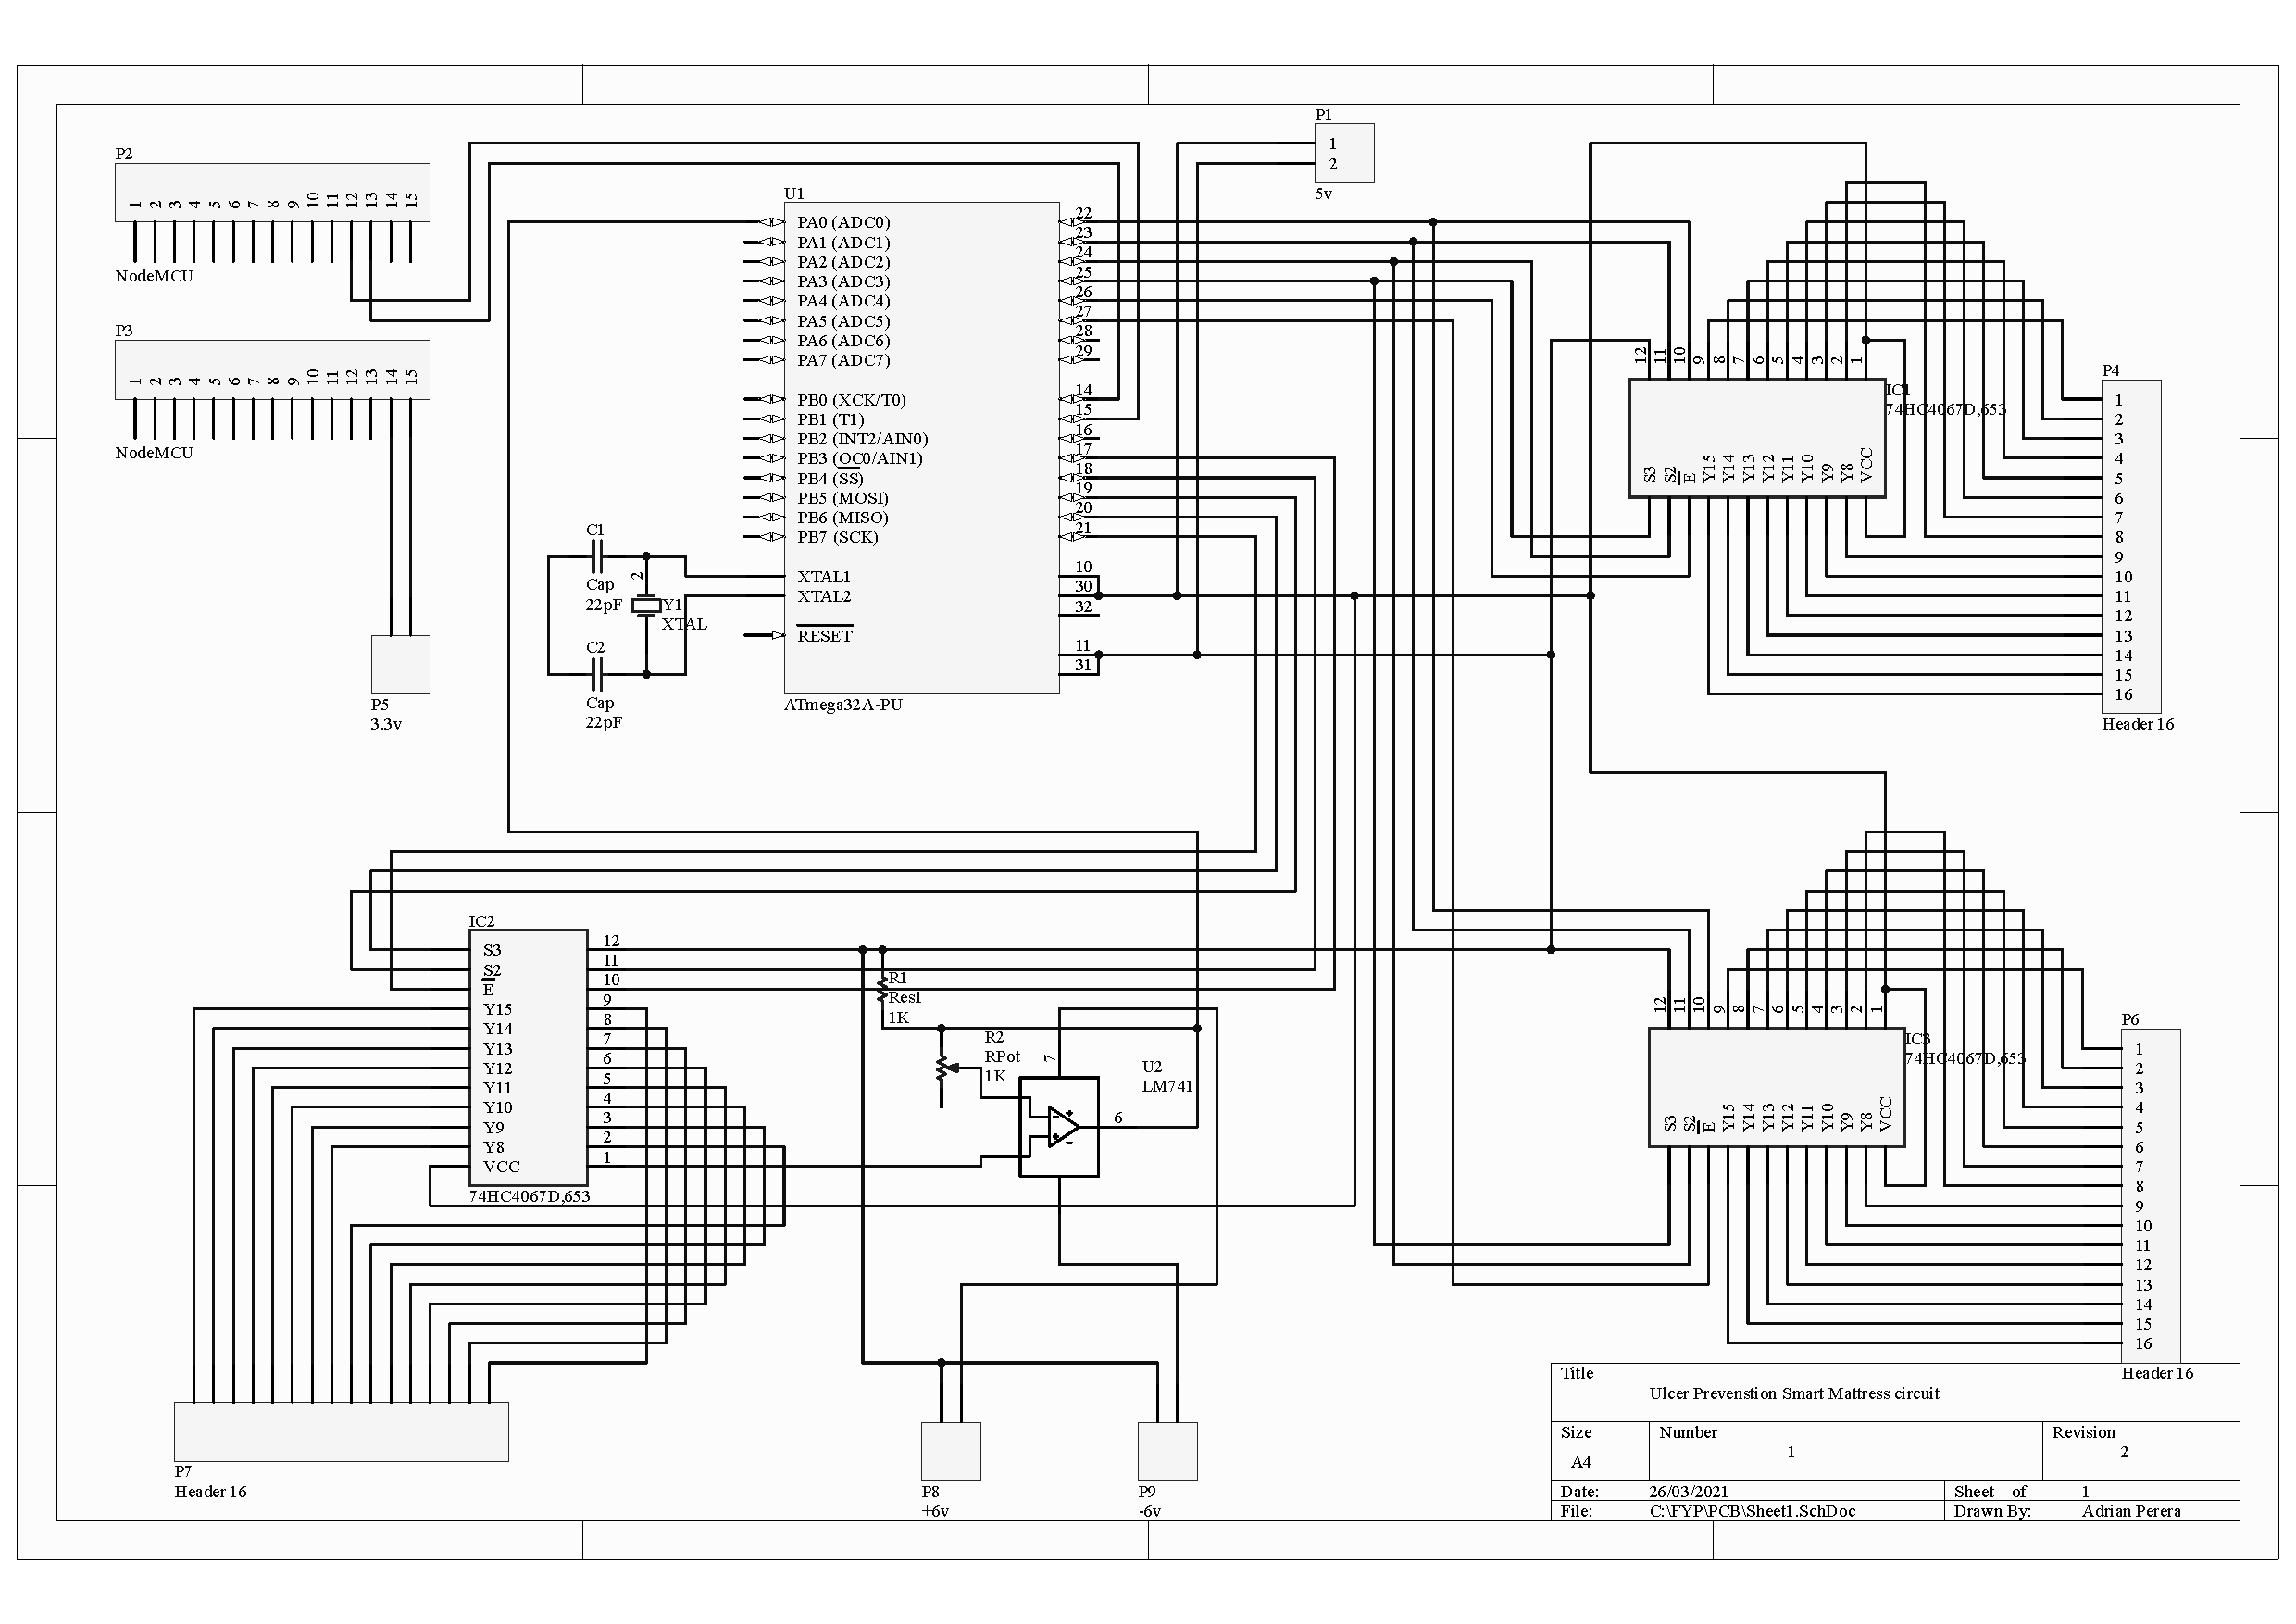
\includegraphics[width=0.8\textheight, angle=90]{figs/schematic1.pdf}
      \caption[Schematic]{Schematic Diagram.}
      \label{fig:schematic}
      \vspace{-1cm}
\end{figure*}


% \textbf{Mean Field Algorithm} \\
% \begin{algorithm*}
  \caption{Inference on Bipartite CRF \label{alg:infer}}
  \begin{algorithmic}[1]
  	  %\Statex
      \State $Q_i(l) \coleq \operatorname{softmax}_i(-\phi_i(l))$ and $R_i(t) \coleq \operatorname{softmax}_i(-\psi_i(t))$\Comment{Initialization}
      \While{not converged}
        \State $Q'_i(l) \minuseq \phi_i(l)$ \Comment{Update due to the first term}
        \State $Q'_i(l) \minuseq \sum_{l' \in \mathcal{L}} \left(\mu(l, l')\sum_{j \neq i}{\Sim_\Phi(i, j)\,Q_j(l')}\right)$ \Comment{Update due to the second term}
        
        \State $R'_i(t) \minuseq \psi_i(t)$ \Comment{Update due to the third term}
        \State $R'_i(t) \minuseq \sum_{t' \in \mathcal{T}} \left([t \neq t']\sum_{j \neq i}{\Sim_\Psi(i, j)\,R_j(t')}\right)$ \Comment{Update due to the fourth term}
        \State $Q'_i(l) \minuseq \sum_{t \in \mathcal{T}} \Big( f(l, \cl(t))\, R_i(t)\Big)$
        \State $R'_i(t) \minuseq \sum_{l \in \mathcal{L}} \Big( f(l, \cl(t))\, Q_i(l) \Big)$ \Comment{Updates due to the fifth term}

		\State $Q'_i(l) \minuseq \sum_{t \in \mathcal{T}} \left( f(l, \cl(t))\, \sum_{j \neq i}{\Sim_\Omega(i, j)\,R_j(t')} \right)$
		\State $R'_i(t) \minuseq \sum_{l \in \mathcal{L}} \left( f(l, \cl(t))\, \sum_{j \neq i}\Sim_\Omega(i, j)\,Q_j(l')\right)$ \Comment{Updates due to the sixth term}
		\State $Q_i(l) \coleq \operatorname{softmax}_i\Big(Q'_i(l)\Big)$ and $R_i(t) \coleq \operatorname{softmax}_i\Big(R'_i(t)\Big)$ \Comment{Normalization}
      \EndWhile
      %\State
  \end{algorithmic}
\end{algorithm*} 



\chapter*{Appendix III}
\addcontentsline{toc}{chapter}{Appendix III}
\label{chapter:appendix3}

ATMega code

\cite{Anurag17}